\documentclass[12pt]{article}
\usepackage[utf8]{inputenc}
\usepackage[english]{babel}
\usepackage{geometry}
\usepackage{listings} % for code snippets
\usepackage{xcolor}
\usepackage{graphicx}
\usepackage{titlesec}
\usepackage{hyperref}
\usepackage [autostyle, english = american]{csquotes}
\MakeOuterQuote{"}

% page setup and spacing
\geometry{a4paper, margin=1in}
\setlength{\parindent}{1em}
\setlength{\parskip}{1em}
\renewcommand{\baselinestretch}{1.0}

% colors for code snippet
\definecolor{codegreen}{rgb}{0,0.6,0}
\definecolor{codegray}{rgb}{0.5,0.5,0.5}
\definecolor{codepurple}{rgb}{0.58,0,0.82}
\definecolor{backcolour}{rgb}{0.95,0.95,0.92}

\hypersetup{
    colorlinks=true,
    linkcolor=blue,
    filecolor=magenta,      
    urlcolor=blue,
    % pdftitle={Overleaf Example},
    pdfpagemode=FullScreen,
    }

% code snippet styling
\lstdefinestyle{mystyle}{
    backgroundcolor=\color{backcolour},   
    commentstyle=\color{codegreen},
    keywordstyle=\color{magenta},
    numberstyle=\tiny\color{codegray},
    stringstyle=\color{codepurple},
    basicstyle=\ttfamily\footnotesize,
    breakatwhitespace=false,         
    breaklines=true,                 
    captionpos=b,                    
    keepspaces=true,                 
    numbers=left,                    
    numbersep=5pt,                  
    showspaces=false,                
    showstringspaces=false,
    showtabs=false,                  
    tabsize=2
}
\lstset{style=mystyle}

\title{ESOF 322: Homework 5}
\author{River Kelly and Peyton Dorsh}
\date{December 2, 2021}

\begin{document}

\maketitle

\newpage
\section*{Question 1 (25 pts)}

\subsection*{a. (10 pts)}
\begin{enumerate}
    \item The system we downloaded was Weka: \url{https://sourceforge.net/projects/weka/}.
    \item This system uses machine learning algorithms to solve data mining problems.
    \item This system has total of 1,871 files in its main java source directory, and a total of 635,973 lines of code.\newline To find the total number of lines, we executed to following command:
\end{enumerate}
\begin{lstlisting}
find . -type f -name "*.java" | xargs wc -l
\end{lstlisting}

\newpage
\subsection*{b. (15 pts)}

\subsubsection*{1. Capture the output of the tool (without checking the “Search in file content” box) and print it.}
\begin{lstlisting}
Found 17 files that possibly contain design patterns.

C:\Users\peyto\Documents\CSCI\Fall2021\esof322\WEKA-SRC\src\main\java\weka\core\CommandlineRunnable.java
Possible patterns: Command

C:\Users\peyto\Documents\CSCI\Fall2021\esof322\WEKA-SRC\src\main\java\weka\core\DictionaryBuilder.java
Possible patterns: Builder

C:\Users\peyto\Documents\CSCI\Fall2021\esof322\WEKA-SRC\src\main\java\weka\core\pmml\PMMLFactory.java
Possible patterns: Factory

C:\Users\peyto\Documents\CSCI\Fall2021\esof322\WEKA-SRC\src\main\java\weka\core\pmml\jaxbbindings\MISSINGVALUESTRATEGY.java
Possible patterns: Strategy

C:\Users\peyto\Documents\CSCI\Fall2021\esof322\WEKA-SRC\src\main\java\weka\core\pmml\jaxbbindings\NOTRUECHILDSTRATEGY.java
Possible patterns: Strategy

C:\Users\peyto\Documents\CSCI\Fall2021\esof322\WEKA-SRC\src\main\java\weka\core\pmml\jaxbbindings\ObjectFactory.java
Possible patterns: Factory

C:\Users\peyto\Documents\CSCI\Fall2021\esof322\WEKA-SRC\src\main\java\weka\experiment\InstanceQueryAdapter.java
Possible patterns: Adapter

C:\Users\peyto\Documents\CSCI\Fall2021\esof322\WEKA-SRC\src\main\java\weka\gui\experiment\GeneratorPropertyIteratorPanel.java
Possible patterns: Iterator

C:\Users\peyto\Documents\CSCI\Fall2021\esof322\WEKA-SRC\src\main\java\weka\gui\knowledgeflow\AbstractGraphicalCommand.java
Possible patterns: Command

C:\Users\peyto\Documents\CSCI\Fall2021\esof322\WEKA-SRC\src\main\java\weka\gui\knowledgeflow\GetPerspectiveNamesGraphicalCommand.java
Possible patterns: Command

C:\Users\peyto\Documents\CSCI\Fall2021\esof322\WEKA-SRC\src\main\java\weka\gui\knowledgeflow\GraphicalEnvironmentCommandHandler.java
Possible patterns: Command

C:\Users\peyto\Documents\CSCI\Fall2021\esof322\WEKA-SRC\src\main\java\weka\gui\knowledgeflow\KFGraphicalEnvironmentCommandHandler.java
Possible patterns: Command

C:\Users\peyto\Documents\CSCI\Fall2021\esof322\WEKA-SRC\src\main\java\weka\gui\knowledgeflow\SendToPerspectiveGraphicalCommand.java
Possible patterns: Command

C:\Users\peyto\Documents\CSCI\Fall2021\esof322\WEKA-SRC\src\main\java\weka\gui\knowledgeflow\TemplateManager.java
Possible patterns: Template

C:\Users\peyto\Documents\CSCI\Fall2021\esof322\WEKA-SRC\src\main\java\weka\gui\simplecli\AbstractCommand.java
Possible patterns: Command

C:\Users\peyto\Documents\CSCI\Fall2021\esof322\WEKA-SRC\src\main\java\weka\knowledgeflow\steps\ASSearchStrategy.java
Possible patterns: Strategy

C:\Users\peyto\Documents\CSCI\Fall2021\esof322\WEKA-SRC\src\test\java\weka\core\DictionaryBuilderTest.java
Possible patterns: Builder
\end{lstlisting}

\subsubsection*{2. How does this tool look for instances of design patterns?}

For instance of design patterns, this tool scanned each of the filenames for design pattern conventions. This is because we did NOT select "Search in File Content". Looking at the results of the capture output, you will notice that the Java files that were matched contain the common design patterns naming conventions.

\subsubsection*{3. Do you think the process used by the tool is correct?  How would you do it? Be specific.}

We believe the process used by this tool is somewhat accurate. Considering that the tool only matched design pattern files based on common naming conventions, it would be safe to assume that the authors of this open source project consciously named such files with the intention of using a specific design pattern.

To better improve the detection of an observed design patterns, we would have to search the contents of each file. Doing so would provide us a greater understanding of the data model represented within the code. We would be able to detect the association between objects (i.e. files), and examine the routine behavior of how these files interact with one another. Doing so would better present the ability of detecting the use of certain design patterns in the project's code. We would identify a used design pattern based on class inheritance and abstraction.

\newpage
\section*{Question 2 (10 pts)}

\begin{center}
    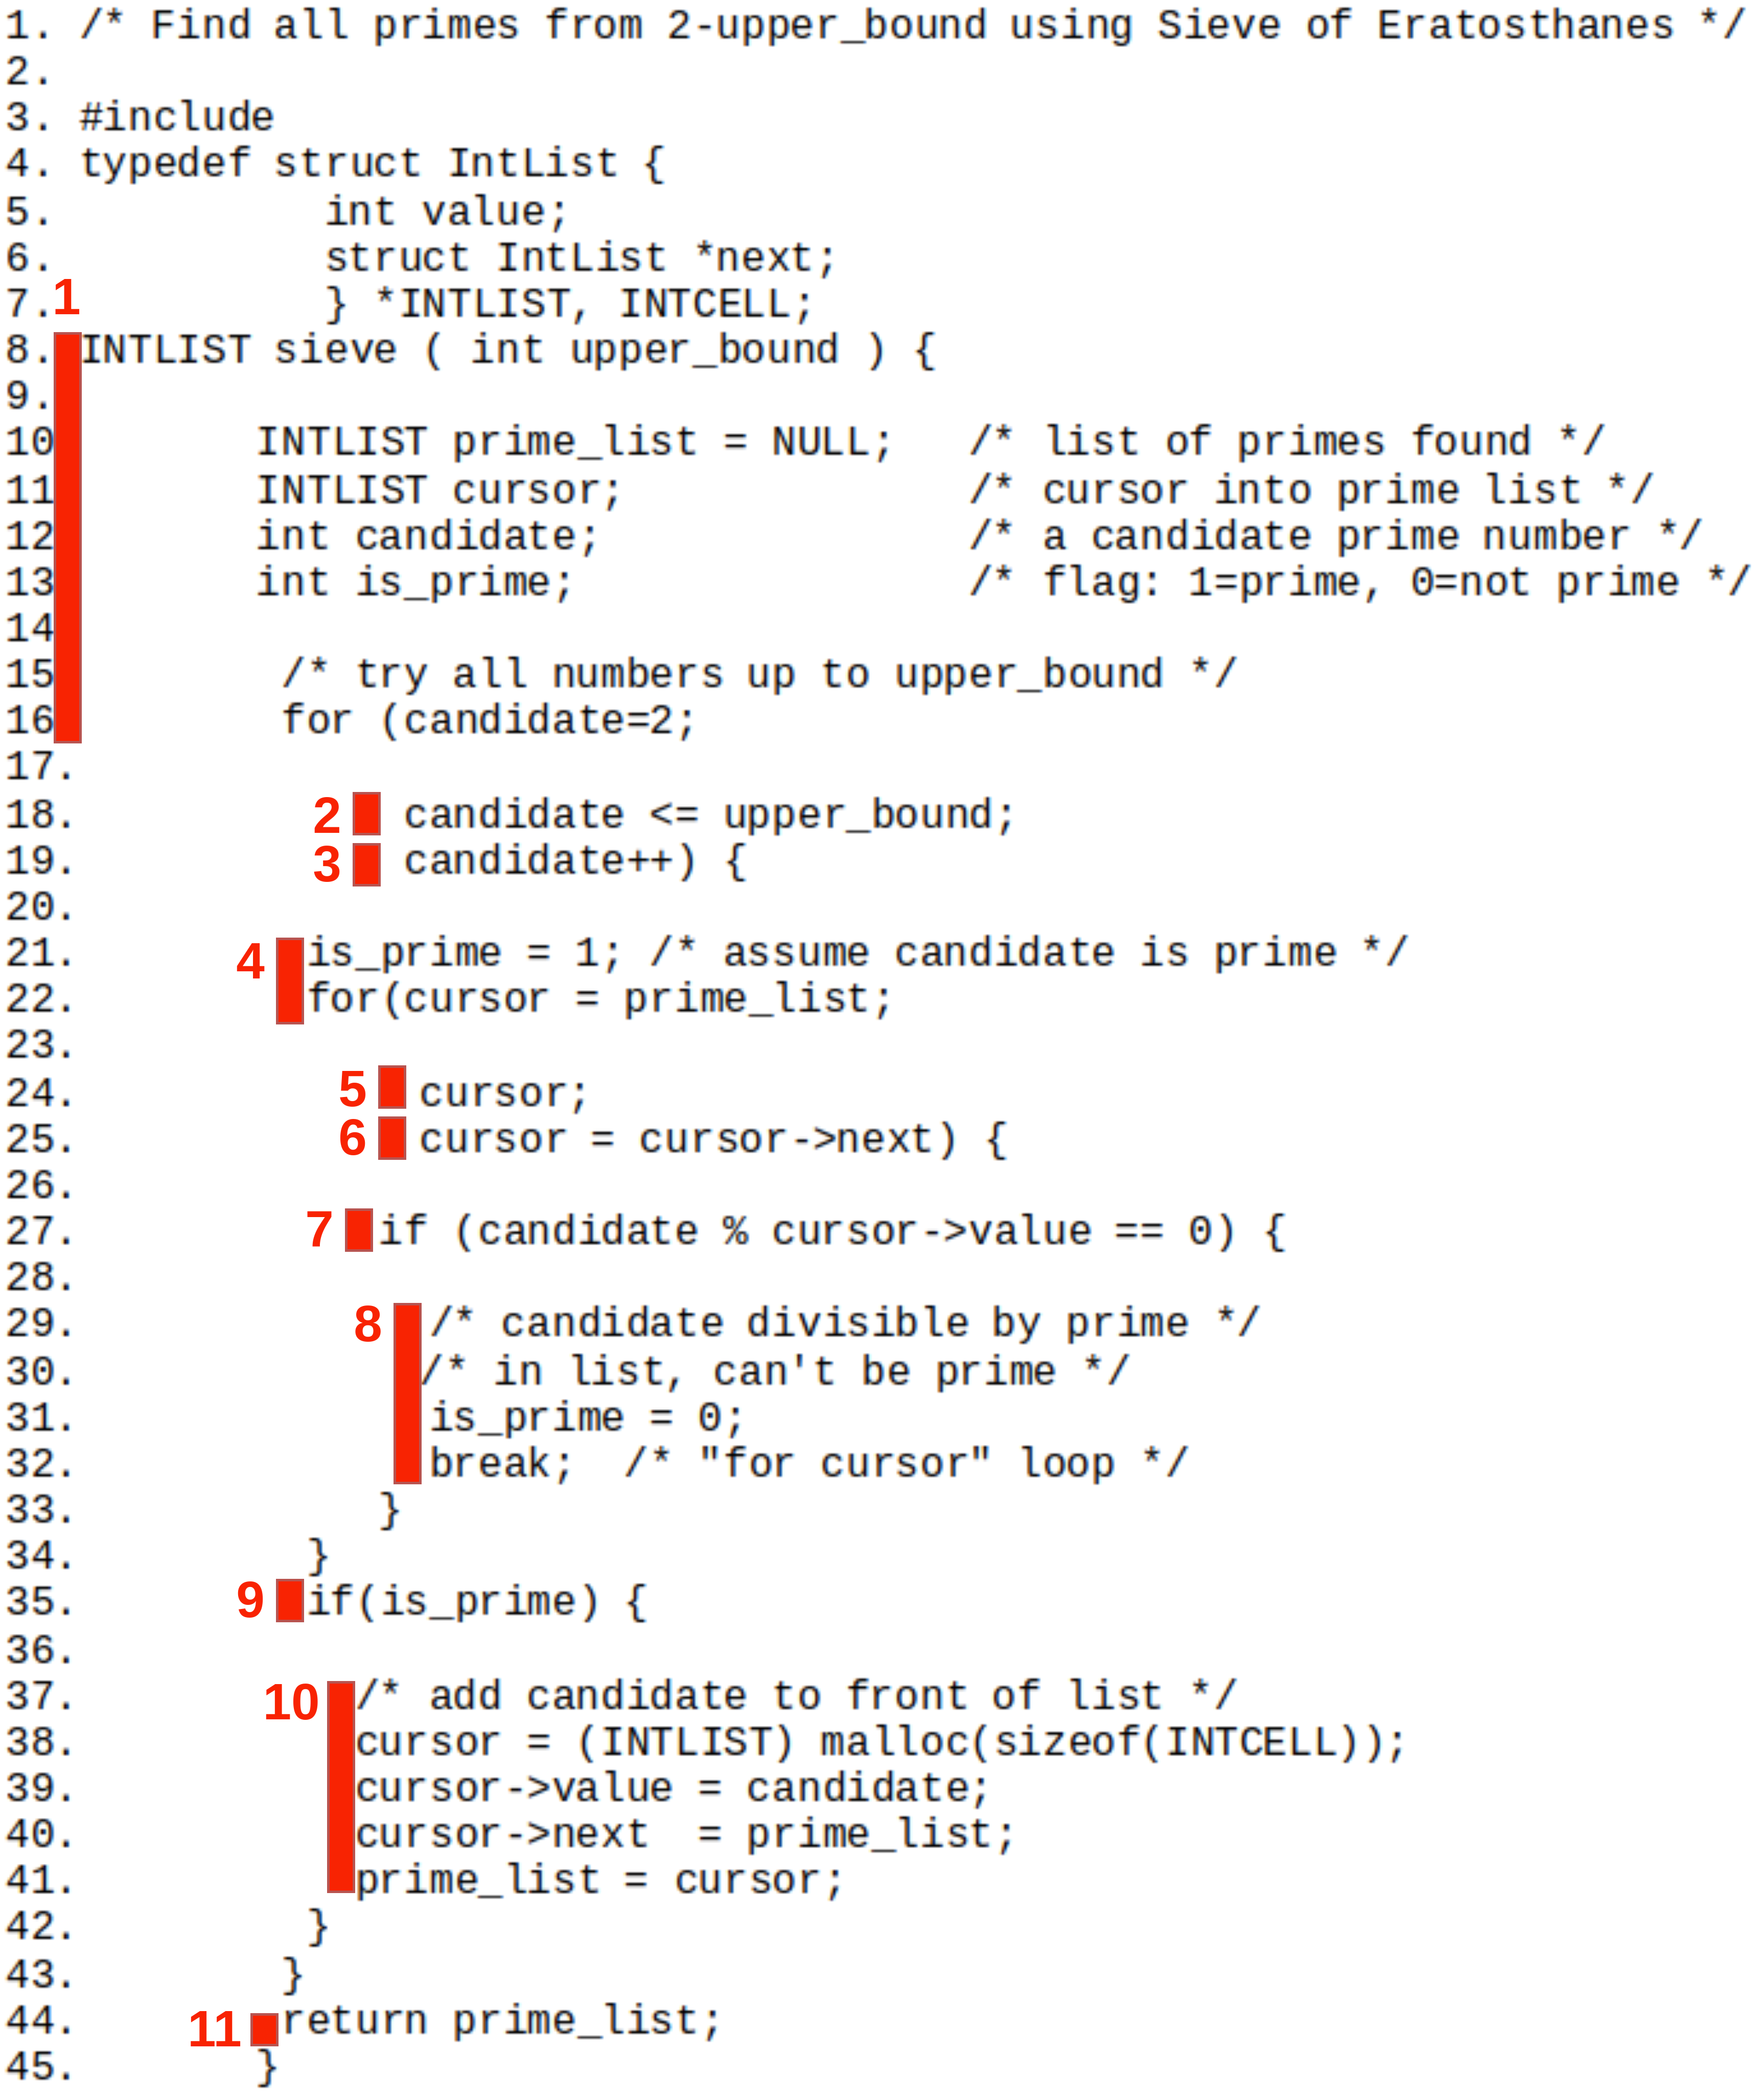
\includegraphics[width=\columnwidth]{q2-a-code-blocks.png}
\end{center}

\begin{center}
    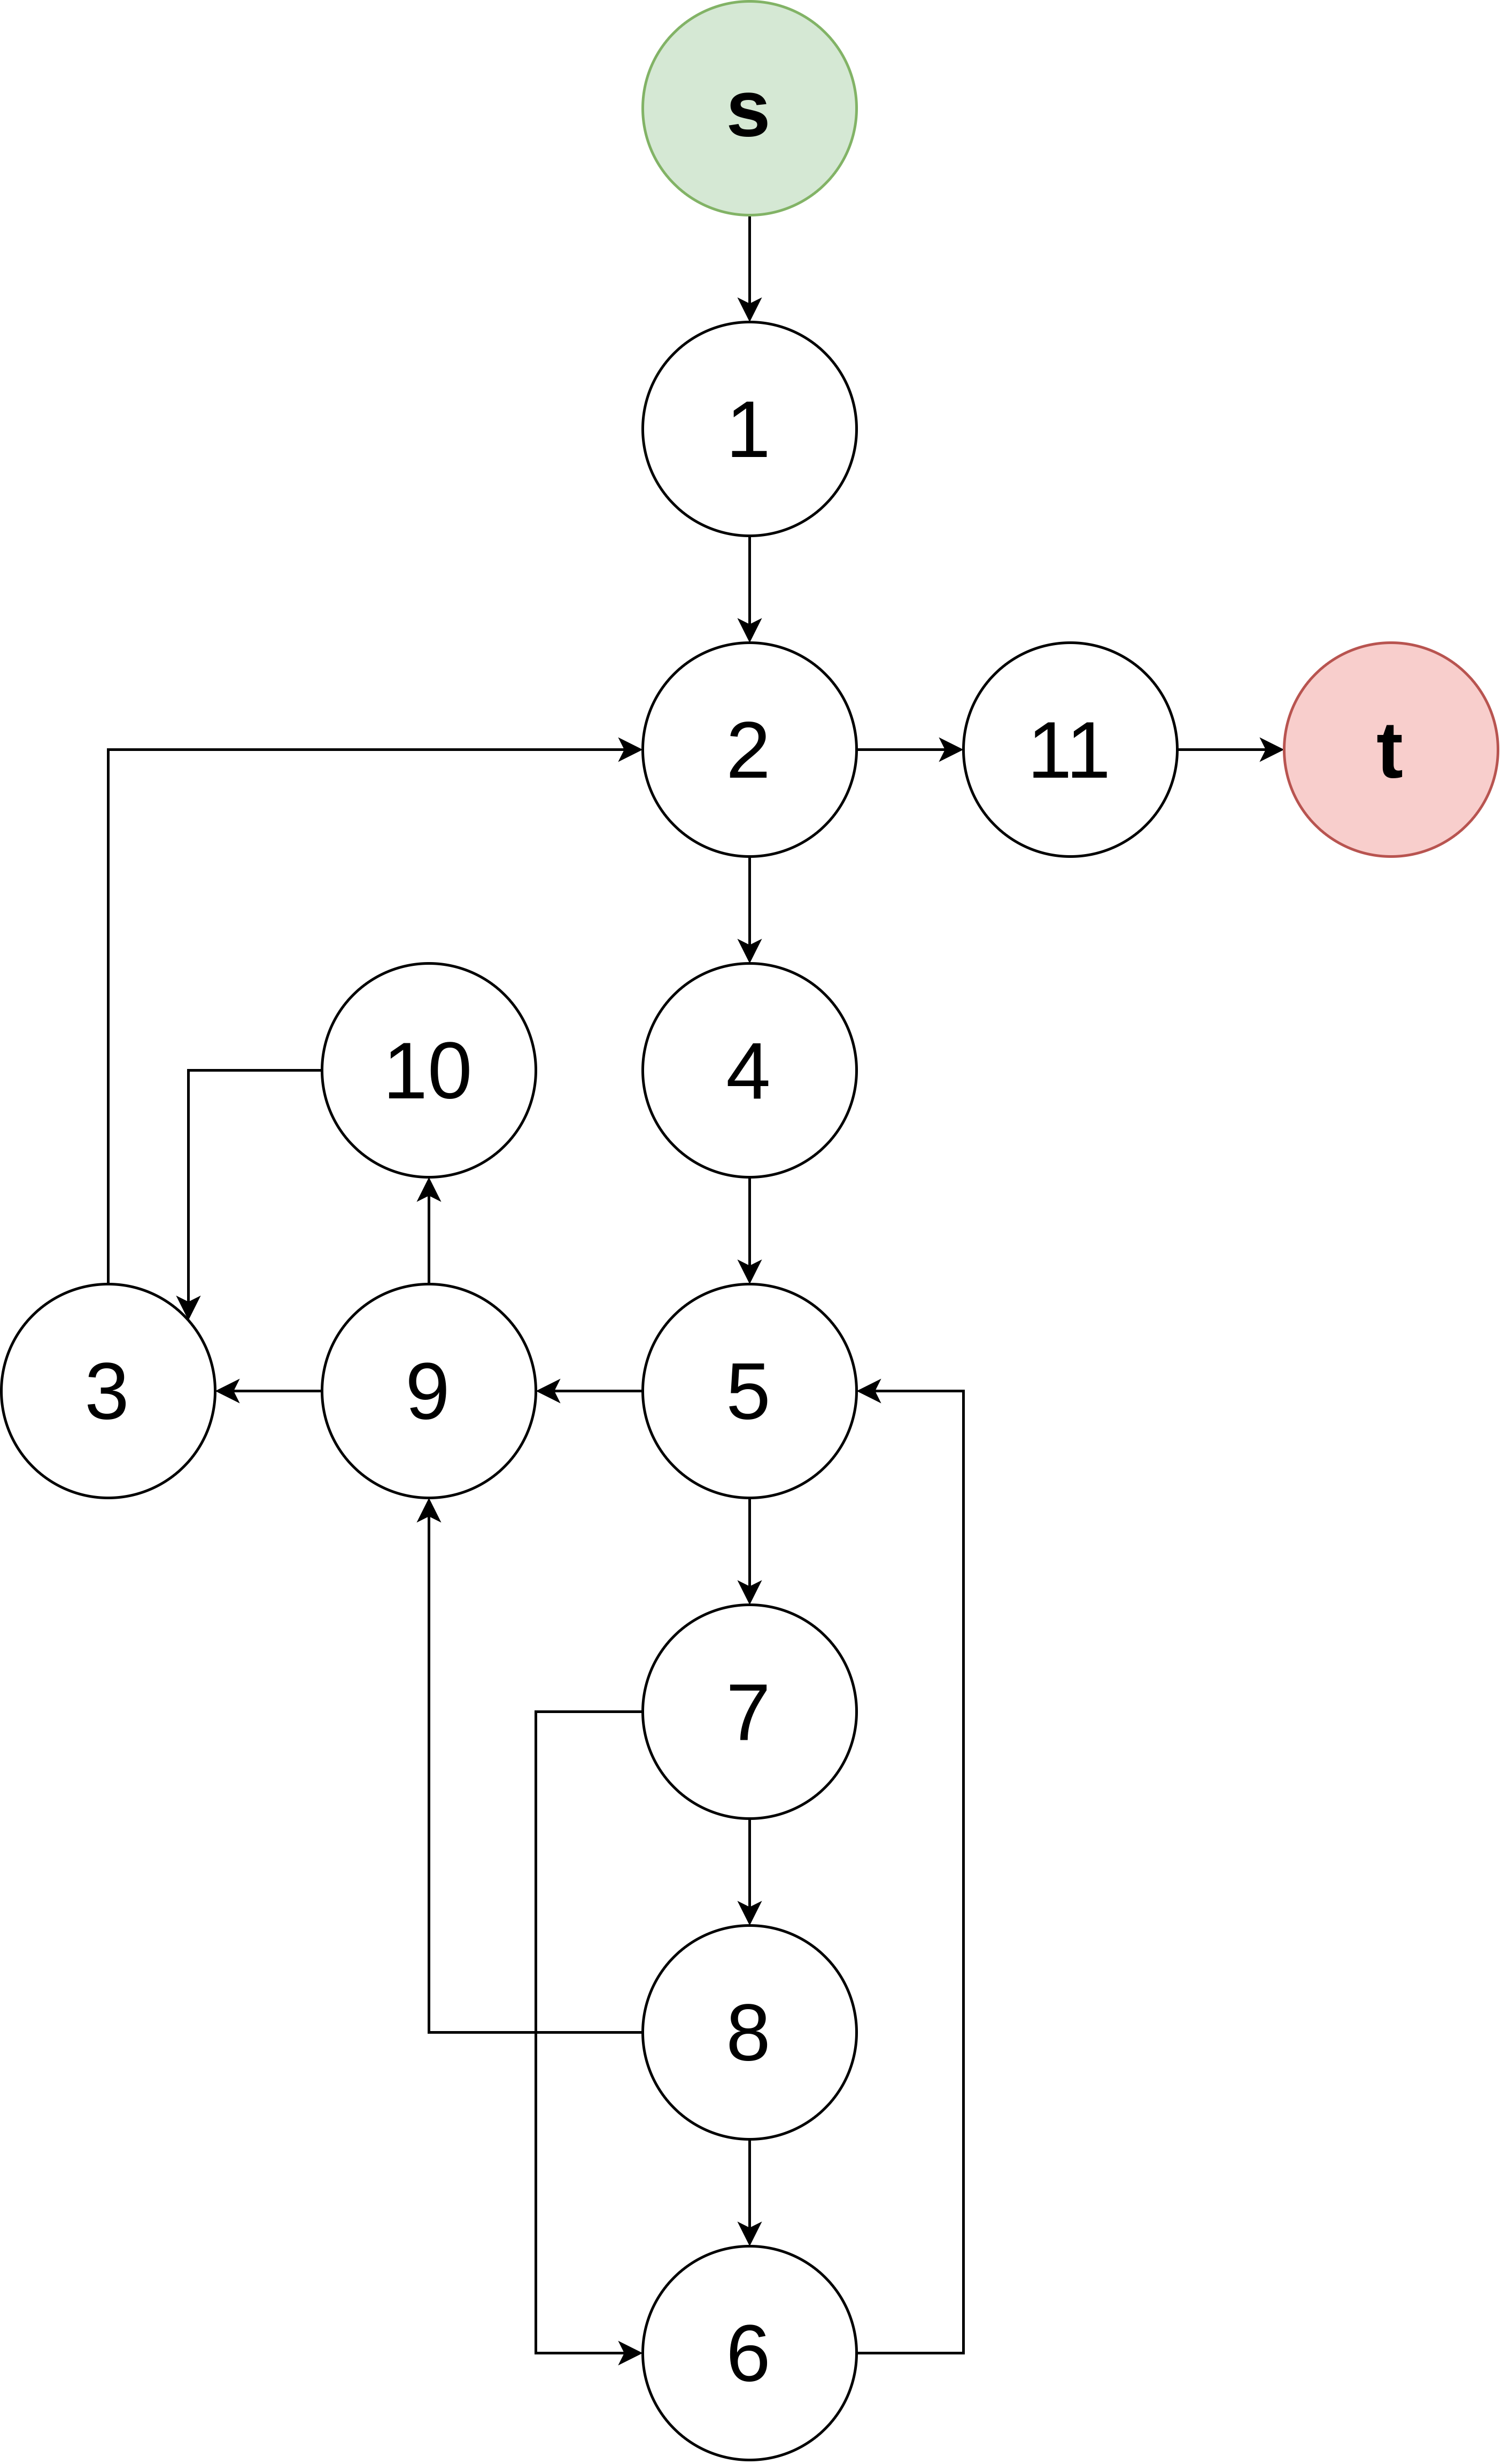
\includegraphics[width=.5\linewidth]{q2-flow-graph.png}
\end{center}

\subsection*{1. Test cases that would give 100\% Node Coverage (NC)}


$T = \{ \newline 
\indent t_{1} = \{s, 1, 2, 4, 5, 7, 8, 6, 5, 9, 3, 2, 11, t\}, \newline
\indent t_{2} = \{s, 1, 2, 4, 5, 9, 10, 3, 2, 11, t\} \newline
\}$

\subsection*{2. Test cases that would give 100\% Edge Coverage (EC)}

$T = \{ \newline 
\indent t_{1} = \{s, 1, 2, 4, 5, 7, 6, 5, 9, 3, 2, 11, t\}, \newline
\indent t_{2} = \{s, 1, 2, 4, 5, 7, 8, 6, 5, 9, 3, 2, 11, t\}, \newline
\indent t_{3} = \{s, 1, 2, 4, 5, 7, 8, 9, 3, 2, 11, t\}, \newline
\indent t_{4} = \{s, 1, 2, 4, 5, 9, 10, 3, 2, 11, t\} \newline
\}$

\subsection*{3. Is 100\% NC or 100\% EC possible in general? Why, or why not?}

Generally speaking, 100\% node coverage and 100\% edge coverage is possible, but speaking practically that is not always the case. Because the set of tests is finite for a given domain, brute force tells us that we could exhaust all potential circumstances. But, the first thing you learn after learning brute force, is that it is typically the worst way of doing things. As computer scientists, we strive for efficiency. In terms of the set of "real-world" tests, this would imply that we provide test cases which are practical, not absolutely encompassing.

\newpage
\section*{Question 3 (10 pts)}

The application we chose to test was YouTube (\url{https://www.youtube.com/}). The scope of our test was videos related to reading sheet music. In out Metamorphic Testing, we began by generating a initial test (base-case) using the search string "\textit{read sheet music}". Then, for each of our Metamorphic Relations we slightly altered the query string and compared the results.

We hypothesize that when searching for a video you YouTube, a user will most likely click on one of the videos suggested on the initial preview (i.e. without scrolling down). To classify a Metamorphic Relation in our test as passing, we required that at least 2 videos shown in the initial test must be shown in the MR to pass, otherwise the MR test was considered a failure.

\subsection*{MR tests preview}

\begin{enumerate}
    \item \textbf{MR \#1}: pass - Query String: \textit{"how to read sheet music"}
    \item \textbf{MR \#2}: fail - Query String: \textit{"reading sheet music"}
    \item \textbf{MR \#3}: pass - Query String: \textit{"read" "sheet" "music"}
\end{enumerate}

\subsection*{Initial Test}

The query string used: "\textit{read sheet music}"

\begin{center}
    
\includegraphics[width=0.5\columnwidth]{q3-initial-test.png}
\end{center}

\newpage
\subsection*{Metamorphic Relations}

\subsubsection*{MR\#1}

\noindent
\textbf{Justification:} We justified that adding the string "how to" before "read sheet music" should be implied implicity considering the scope of our test (i.e. a user wishing to learn 'how to' read sheet music).

\noindent
\textbf{Query String:} "\textit{how to read sheet music}"

\begin{center}
    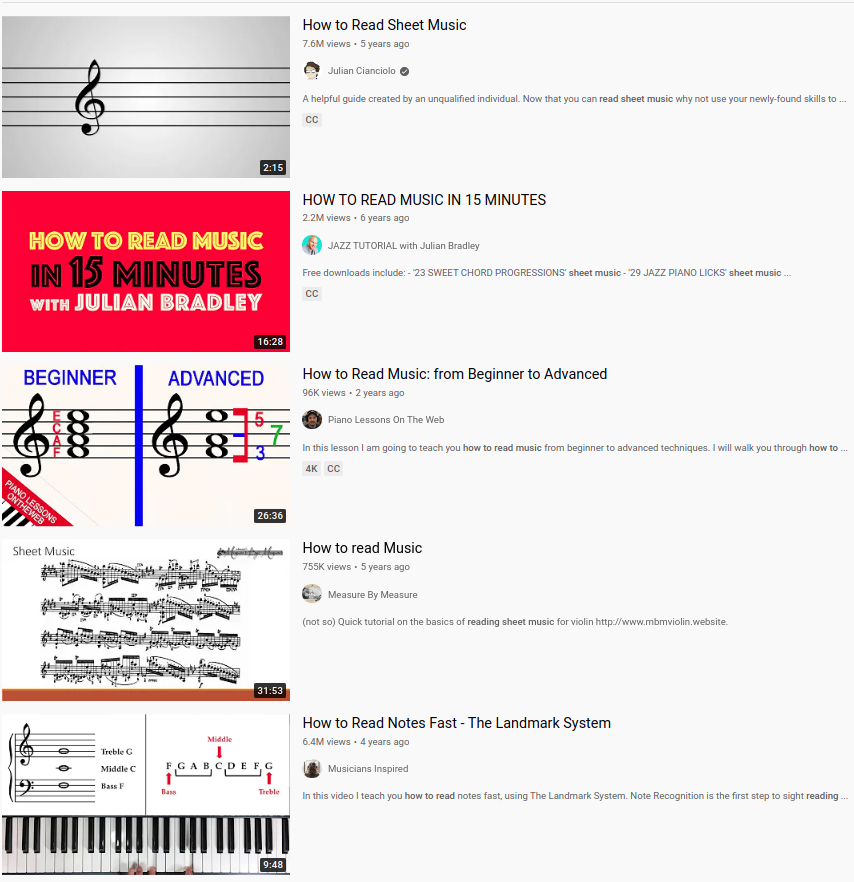
\includegraphics[width=0.5\columnwidth]{q3-mr1.png}
\end{center}

\newpage
\subsubsection*{MR\#2}

\noindent
\textbf{Justification:} From our original phrase, we changed the verbal tense of the word "read" to "reading". We concluded that this modification should not alter the search results.

\noindent
\textbf{Query String:} \textit{"reading sheet music"}

\begin{center}
    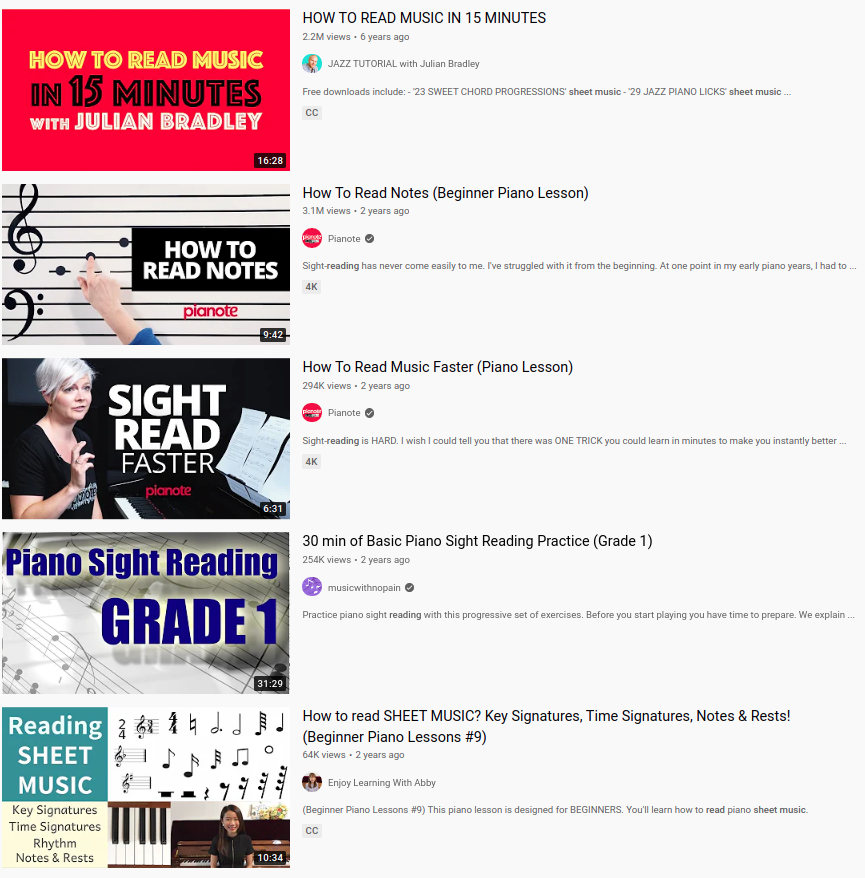
\includegraphics[width=0.5\columnwidth]{q3-mr2.png}
\end{center}

\newpage
\subsubsection*{MR\#3}

\noindent
\textbf{Justification:} We added quotes around each of the words from the original phrase.

\noindent
\textbf{Query String:} \textit{"read" "sheet" "music"}

\begin{center}
    
\includegraphics[width=0.5\columnwidth]{q3-mr3.png}
\end{center}


\newpage
\section*{Question 4 (12 pts)}

\begin{enumerate}
    \item Line 6: if $(i < 1 )$\newline Test case $i = 1$ will kill this mutant.
    \item Line 6: if $( i == 1 )$\newline Test case $i = 0$ will kill this mutant.
    \item Line 12: $fib2 = fib$;\newline Test case $i = 3$ will kill this mutant.
\end{enumerate}

\end{document}